\documentclass[../main/main.tex]{subfiles}

% Put everything that shall appear in the method
% inside this document environment.
\begin{document}
	
	\textbf{Task: describe your ideas and your realization of the task}
	
	\subsection{Designing the Questionnaire (MAG)}
	
	We started out by designing a questionnaire in \LaTeX and using the corporate design of our university. We separated each task clearly from the one another and wrote the instructions in the headline. The body of each tasks consists of task related information on the left, space for the answer in the middle and an empty coordinate system on the right. It was important to us to keep this structure to increase reliability across the tasks.
	
	We decided to use sorting tasks, because of their high objectivity (see section \ref{sec:discussion} for a discussion on question types). The first seven tasks were closed-form sorting tasks. Directly after executing each task, the subjects were asked to fill out the coordinate system with a probability density function over their performance. We decided to ask the subjects to sort five terms in a predefined order. We decided to use two easy items, three medium and two hard items. We randomized the location of the items as well as the order of the answer possibilities. An example can be seen in figure \ref{fig:example-task}.
	
	\begin{figure}[h]
		\label{fig:example-task}
		\centering
		\captionsetup{justification=centering}
		\fbox{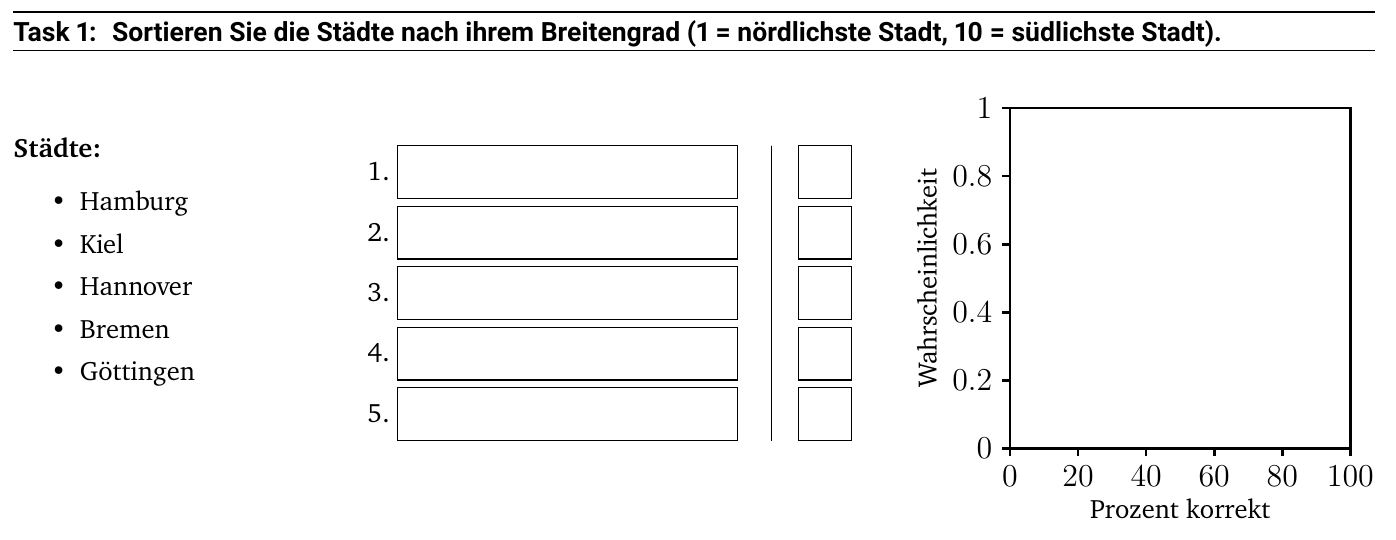
\includegraphics[width=.8\textwidth]{../assets/example-task-1.png}}
		\caption{Example closed-form sorting task.}
	\end{figure} 
	
	After the seven tasks, we asked the subjects to estimate their performance over all the previous tasks, by drawing another probability density function. With this we want to learn how well humans can average their performance on several task. 
		
	 The eighth task was an open end sorting tasks, which we decided to incorporate out of curiosity how the self-assessment would change in comparison to closed form sorting tasks. The task can be seen in figure \ref{fig:example-task2}.
	 
	 \begin{figure}[h]
	 	\label{fig:example-task2}
	 	\centering
	 	\captionsetup{justification=centering}
	 	\fbox{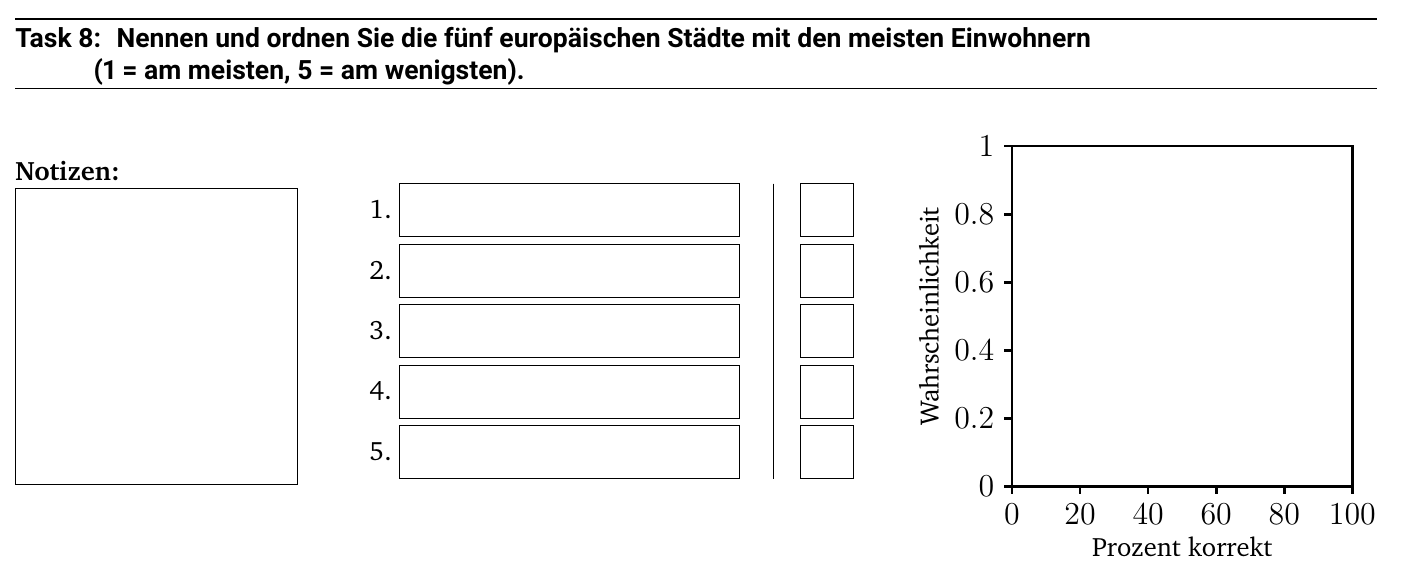
\includegraphics[width=.8\textwidth]{../assets/example-task-8.png}}
	 	\caption{Example open end sorting task.}
 	\end{figure} 
	 

	\subsection{Processing Pipeline (MAG)}
	
	\begin{center}
	\begin{tikzpicture}
		\label{fig:processing}
		% PDF box
		\node[rectangle, draw=black, rounded corners=2mm, minimum width=3cm, minimum height=1cm, line width=1pt] 
		at (-0.6, 10) {\Large PDF file};
		
		% PDF arrow
		\draw[thick,arrows={-open triangle 45}]  (-7, 10) -- node [pos=.5, above] {scan questionnaire} (-2.4, 10);
		
		\draw[thick,arrows={-triangle 45}]  (-0.6, 9.4) -- (-0.6, 8.6);
		
		% JPG box
		\node[rectangle, draw=black, rounded corners=2mm, minimum width=3cm, minimum height=1cm, line width=1pt]  (jpgbox)
		at (-0.6,8) {\Large JPG};
		
		% JPG arrow
		\draw[thick,arrows={-open triangle 45}]  (-7, 8) -- node [pos=.5, above] {photograph questionnaire} (-2.4, 8);
		
		\node[inner sep=0pt] (dist1) at (-5.5,4.8)
		{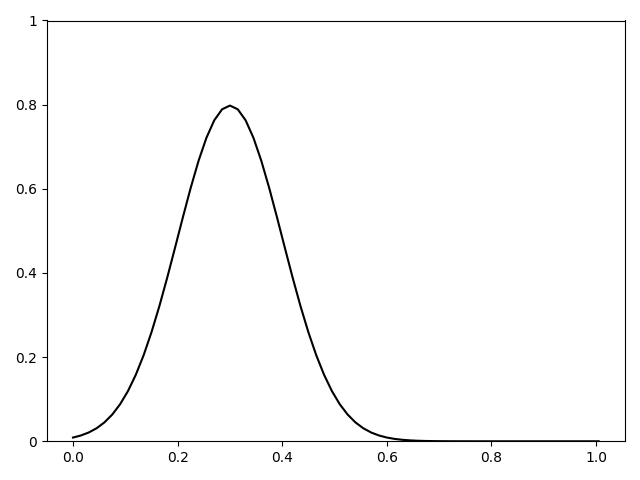
\includegraphics[width=.33\textwidth]{../assets/example_distribution_1.png}};
		
		\node[inner sep=0pt] (dist2) at (-0.6,4.8)
		{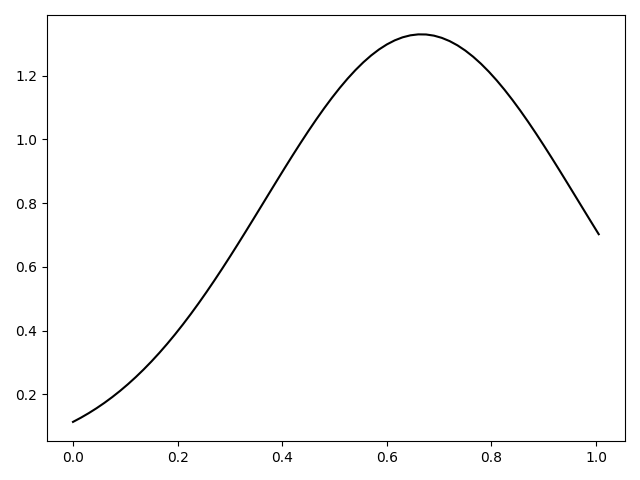
\includegraphics[width=.33\textwidth]{../assets/example_distribution_2.png}};
		
		\node[inner sep=0pt] (dist3) at (5,4.8)
		{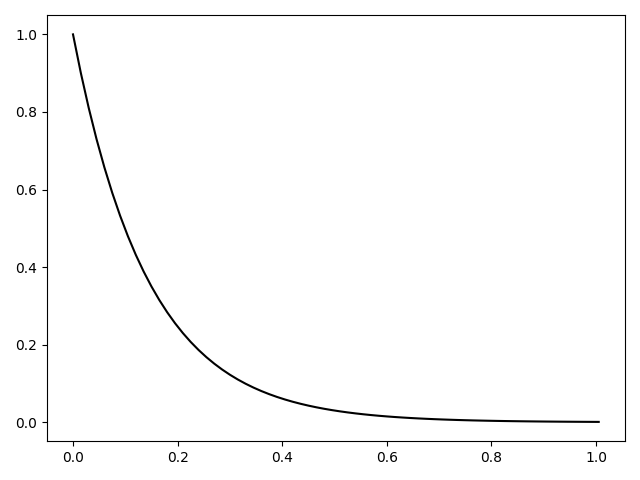
\includegraphics[width=.33\textwidth]{../assets/example_distribution_3.png}};
		
		\node at (2.2, 4.8) {\Huge ...};
		
		\draw[thick,arrows={-triangle 45}]  (-0.6, 7.4) -- (-0.6, 7) -- (-5.5, 7) -- (-5.5, 6.5);
		\draw[thick,arrows={-triangle 45}]  (-0.6, 7.4) -- (-0.6, 7) -- (-0.6, 7) -- (-0.6, 6.5);	
		\draw[thick,arrows={-triangle 45}]  (-0.6, 7.4) -- (-0.6, 7) -- (5, 7) -- (5, 6.5);
		
		\node[inner sep=0pt] (dist1) at (-5.5,0.5)
		{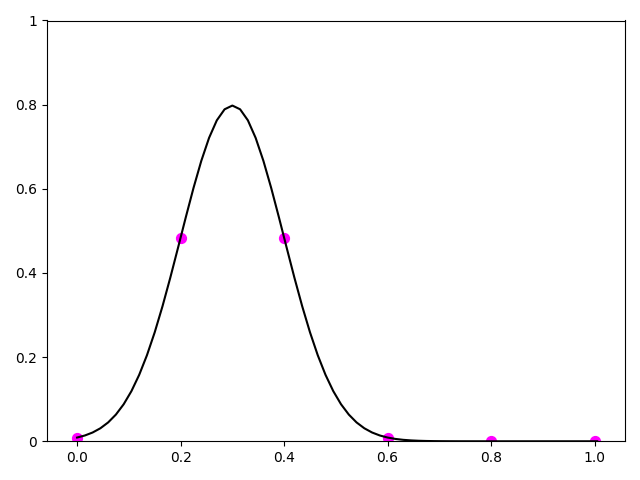
\includegraphics[width=.33\textwidth]{../assets/example_distribution_1_points.png}};
		
		\node[inner sep=0pt] (dist2) at (-0.6,0.5)
		{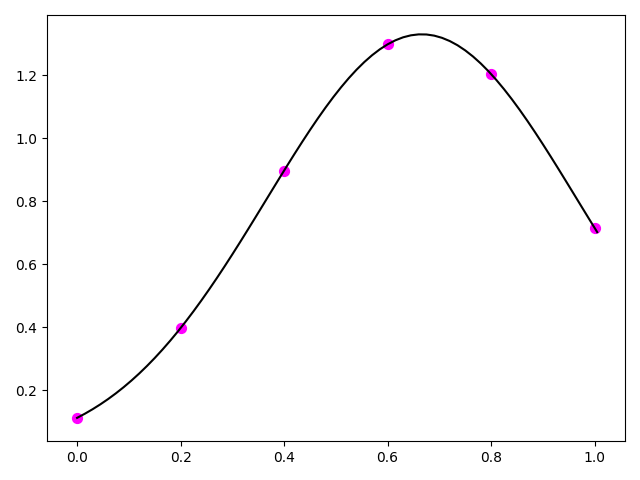
\includegraphics[width=.33\textwidth]{../assets/example_distribution_2_points.png}};
		
		\node[inner sep=0pt] (dist3) at (5,0.5)
		{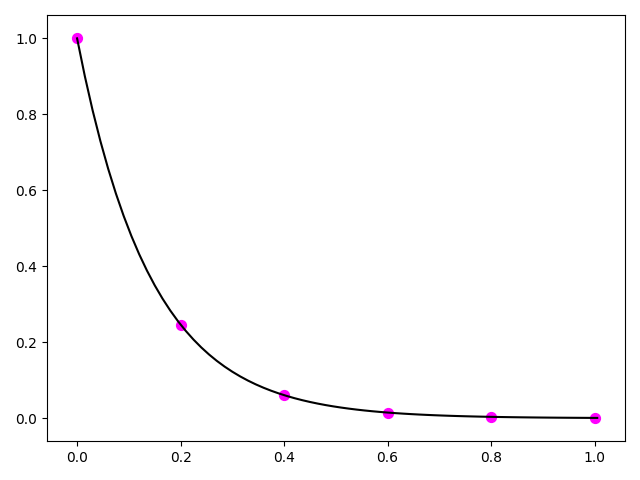
\includegraphics[width=.33\textwidth]{../assets/example_distribution_3_points.png}};
		
		\node at (2.2, 0.5) {\Huge ...};
		
		\draw[thick,arrows={-triangle 45}]  (-5.5, 3) -- (-5.5, 2.2);
		\draw[thick,arrows={-triangle 45}]  (-0.6, 3) -- (-0.6, 2.2);	
		\draw[thick,arrows={-triangle 45}]  (5, 3) -- (5, 2.2);
		
		\draw[thick,arrows={-triangle 45}]  (-5.5, -1.4) -- (-5.5, -1.8) -- (-0.9, -1.8) -- (-0.9, -2.4);
		\draw[thick,arrows={-triangle 45}]  (-0.6, -1.4) -- (-0.6, -1.8) -- (-0.6, -1.8) -- (-0.6, -2.4);
		\draw[thick,arrows={-triangle 45}]  (5, -1.4) -- (5, -1.8) -- (-0.3, -1.8) -- (-0.3, -2.4);
		
		% Discrete box
		\node[rectangle, draw=black, rounded corners=2mm, minimum width=5cm, minimum height=1cm, line width=1pt]  (discretebox)
		at (-0.6,-3) {\Large Discrete Probability Points};
		
		\draw[thick,arrows={-triangle 45}]  (-0.6, -3.6) -- (-0.6, -4.4);
		
		% Normalize box
		\node[rectangle, draw=black, rounded corners=2mm, minimum width=5cm, minimum height=1cm, line width=1pt]  (normalize)
		at (-0.6,-5) {\Large Normalize};
		
				\draw[thick,arrows={-triangle 45}]  (-0.6, -5.6) -- (-0.6, -6.4);
		
		% Brier score box
		\node[rectangle, double, draw=black, rounded corners=2mm, minimum width=5cm, minimum height=1cm, line width=1pt]  (brier)
		at (-0.6,-7) {\Large Brier Score};
		
				\draw[thick,arrows={-triangle 45}] (-0.6, -8.4) -- (-0.6, -7.6) ;
		
		\node[rectangle, draw=black, rounded corners=2mm, minimum width=5cm, minimum height=1cm, line width=1pt]  (score)
		at (-0.6,-9) {\Large Score Answers};
		
		\draw[thick,arrows={-triangle 45}]  (-0.6, -10.4) -- (-0.6, -9.6) ;
		
		\node[rectangle, draw=black, rounded corners=2mm, minimum width=3cm, minimum height=1cm, line width=1pt]  (score)
		at (-0.6,-11) {\Large CSV};
		
		\draw[thick,arrows={-open triangle 45}]  (-7, -11) -- node[pos=.5, above] {enter answers} (-2.4, -11);
	\end{tikzpicture}
	\end{center}

	The pipeline that we used to process the questionnaire can be seen in the figure above. We start out by digitizing the image. This is important so that we are able to apply computer vision to extract the probability density functions. For convenience we provided two ways: either scan the questionnaire as a PDF file or photograph each page of the questionnaire and upload the pages as JPEG's. In the first case, we use the python package ``pdf2image'' to convert each PDF page into a single JPEG page, which is not necessary in the second case, cause the JPEG's are already available.  

	After the digitization of the questionnaire, the probability density functions are detected on the questionnaire and extracted as single images. From these images we build a digital representation of each probability density functions and read discrete probabilities at the desired locations. Afterwards we normalize the probabilities in order for them to sum to one. This way, the subjects do not need to care about drawing a normalized probability function and can rather concentrate on which area they assign a higher percentage and which areas they assign a lower percentage. 
	
	For a meaningful comparison, we need need to insert the answers of the subjects. We do this by filling a CSV file for each subject by hand. The answers from the CSV file are imported into our program and subsequently scored. An automatic scoring improves the objectivity and avoids errors. Finally, we use the points that each person achieved for each tasks and the normalized probabilities from the probability density functions to calculate the Brier score, which quantifies uncertainties.
	
	The remaining segments of this sections examine the processing pipeline in more detail.
	
	
	\subsection{Extracting Probability Density Functions (MAG)}
	
	To extract the probability density functions from a scanned PDF into an image, we used computer vision to detect the probability density functions on the JPEG and simply cut out the detected regions from the JPEG. The cutout process is fairly easy. In python, images are stored as an array of numbers. As soon as we get the area of the pdf as pixels, we can simply enter these pixel indices in the array and extract that part of the image. Then we save it using OpenCV a free computer vision library in python.
	
	The hard part is to identify the probability density functions in the image. However, we designed our questionnaire in a way that reduces the detection of the pdf to the detection of a big square. If we can reliably detect the coordinate system, which the subjects use to draw their pdfs in, we can extract the pdf if we only look at the pixels which lie inside this square.
	
	To detect squares, we need to detect vertical and horizontal lines first. We did exactly that and looked at all contours that could be build with horizontal and vertical lines. This will output all lines on their own, but also all triangles, rectangles and squares. Everything that forms a contour. Now we sorted the contours. It is important to sort the contours (or later pdfs), regarding their position on the page. To the computer all pdfs look the same, so we have to make sure that we assign the correct pdf to the correct task. Because all tasks are ordered in ascending order, we can sort the pdfs from north to south.
	
	Next, we had to find the correct square from the contours. We did this by iterating over the contours and testing each contour regarding some constraints.
	
	\begin{enumerate}
		\item The horizontal and vertical length of the contour had to be approximately the same length. We allowed for exactly 8\% variation. So one side could be up to 8\% longer than the other side. This factor is necessary, because of the difficulty to scan a paper perfectly aligned.
		\item The coordinate system has a height of 4.5cm. A Din A4 paper is exactly 29.7cm high. This means that each pdf takes about 0.15\% of the height of the image. Allowing for some deviation, the height of the contour had to be between 10 and 20\% of the height of the JPEG. 
		\item The coordinate system has a width of 4.5cm. A Din A4 paper is exactly 21cm wide. This means that each pdf takes about 0.21\% of the width of the image. Allowing for some deviation, the width of the contour had to be between 15 and 25\% of the width of the JPEG. 
		\item Last, we excluded all contours which were lying on the left half of the page.
	\end{enumerate}

	\noindent Constraint 1 makes sure that we find squares. Constraint 2 and 3 make sure we find the squares with the correct size. Constraint 4 makes sure that we do not take any squares from the left side of the page. We designed the questionnaire in a way that all pdfs are located at the right half of the page.
	
	Because we calculate the extraction of the pdfs with percentages relative to the size of a Din A4 paper, it is independent of the DPI and resolution of the scanner or photo camera with which the questionnaire is copied.
	
	\subsection{Extracting Probabilites from probability density functions (YF)}
	
	\subsection{Scoring the answers (YF)}
	
	\subsection{Calculating the Brier Score (YF)}

\end{document}